\documentclass[a4paper,10.5pt]{article}

% ===== 中文支持 =====
% quiet: 抑制 fontspec 的字体提示警告(TeX Live 自带 Fandol otf 缺少 OpenType
%        "CJK" script 标签,会触发无害的 "does not contain requested Script" 警告)
\PassOptionsToPackage{quiet}{fontspec}
% fontset=none: 不使用 ctex 默认 Fandol 字体集(其中 FandolFang 仿宋字形覆盖不全),改为手动指定
\usepackage[UTF8,fontset=none]{ctex}

% ===== 中文字体手动指定 =====
% 避开 FandolFang(仿宋,字形覆盖不全),仿宋族(zhfs/mono)改用 FandolKai 楷体替代
\setCJKmainfont{FandolSong-Regular}[Extension=.otf,BoldFont=FandolSong-Bold,ItalicFont=FandolKai-Regular]
\setCJKsansfont{FandolHei-Regular}[Extension=.otf,BoldFont=FandolHei-Bold]
\setCJKmonofont{FandolKai-Regular}[Extension=.otf]
\setCJKfamilyfont{zhsong}{FandolSong-Regular}[Extension=.otf,BoldFont=FandolSong-Bold]
\setCJKfamilyfont{zhhei}{FandolHei-Regular}[Extension=.otf,BoldFont=FandolHei-Bold]
\setCJKfamilyfont{zhkai}{FandolKai-Regular}[Extension=.otf]
\setCJKfamilyfont{zhfs}{FandolKai-Regular}[Extension=.otf]

% ===== 页面设置 =====
\usepackage[top=1.5cm,bottom=1.5cm,left=1.8cm,right=1.8cm]{geometry}
\usepackage{xcolor}
\usepackage{enumitem}
\usepackage{titlesec}
\usepackage{fontspec}
\usepackage{graphicx}
\usepackage{tabularx}
\usepackage{array}
\usepackage{hyperref}
\usepackage{fontawesome5}

% ===== 颜色定义 =====
\definecolor{themeblue}{RGB}{31, 73, 125}
\definecolor{themered}{RGB}{192, 0, 0}
\definecolor{darkgray}{RGB}{80, 80, 80}

% ===== 超链接设置 =====
\hypersetup{
    colorlinks=true,
    linkcolor=themeblue,
    urlcolor=themeblue
}

% ===== 段落与列表设置 =====
\setlength{\parindent}{0pt}
\setlength{\parskip}{2pt}
\renewcommand{\baselinestretch}{1.15}

% ===== 章节标题样式 =====
\titleformat{\section}
    {\color{themeblue}\Large\bfseries}
    {}{0pt}{}
    [\vspace{-6pt}\color{themeblue}\rule{\textwidth}{1.2pt}]
\titlespacing*{\section}{0pt}{8pt}{4pt}

% ===== 自定义命令 =====
% 教育/工作条目: 4参数 - 学校 | 院系/专业 | 学位 | 时间
\newcommand{\eduentry}[4]{%
    \noindent\textbf{#1} \,|\, #2 \,|\, #3 \hfill \textbf{#4}\par\vspace{2pt}
}

% 项目标题: 编号 + 红色标题 + 说明
\newcommand{\projitem}[3]{%
    \item[\textbf{\color{themered}#1.}] \textcolor{themered}{\textbf{#2}}: #3
}

% 子条目 (\subitem 是 LaTeX 内核命令,改名避免冲突)
\newcommand{\subproj}[2]{%
    \par\vspace{2pt}\noindent\textbf{#1} #2\par
}

% ===== 列表全局设置 =====
\setlist[itemize]{leftmargin=*,topsep=2pt,itemsep=2pt,parsep=0pt}
\setlist[enumerate]{leftmargin=*,topsep=2pt,itemsep=4pt,parsep=0pt}

\begin{document}

% ===================== 个人信息 =====================
\begin{minipage}[c]{0.78\textwidth}
    \vspace{0pt}
    \begin{center}
        {\Huge\bfseries 薛景秦}\\[6pt]
        {\small 15110309796 \,|\, \href{mailto:xuejingqin@ihep.ac.cn}{xuejingqin@ihep.ac.cn}}
    \end{center}
\end{minipage}%
\begin{minipage}[c]{0.20\textwidth}
    \vspace{0pt}
    \hfill
    % 同时锁定宽高,使照片正好填满方框(2.8cm x 3.6cm)
    \fbox{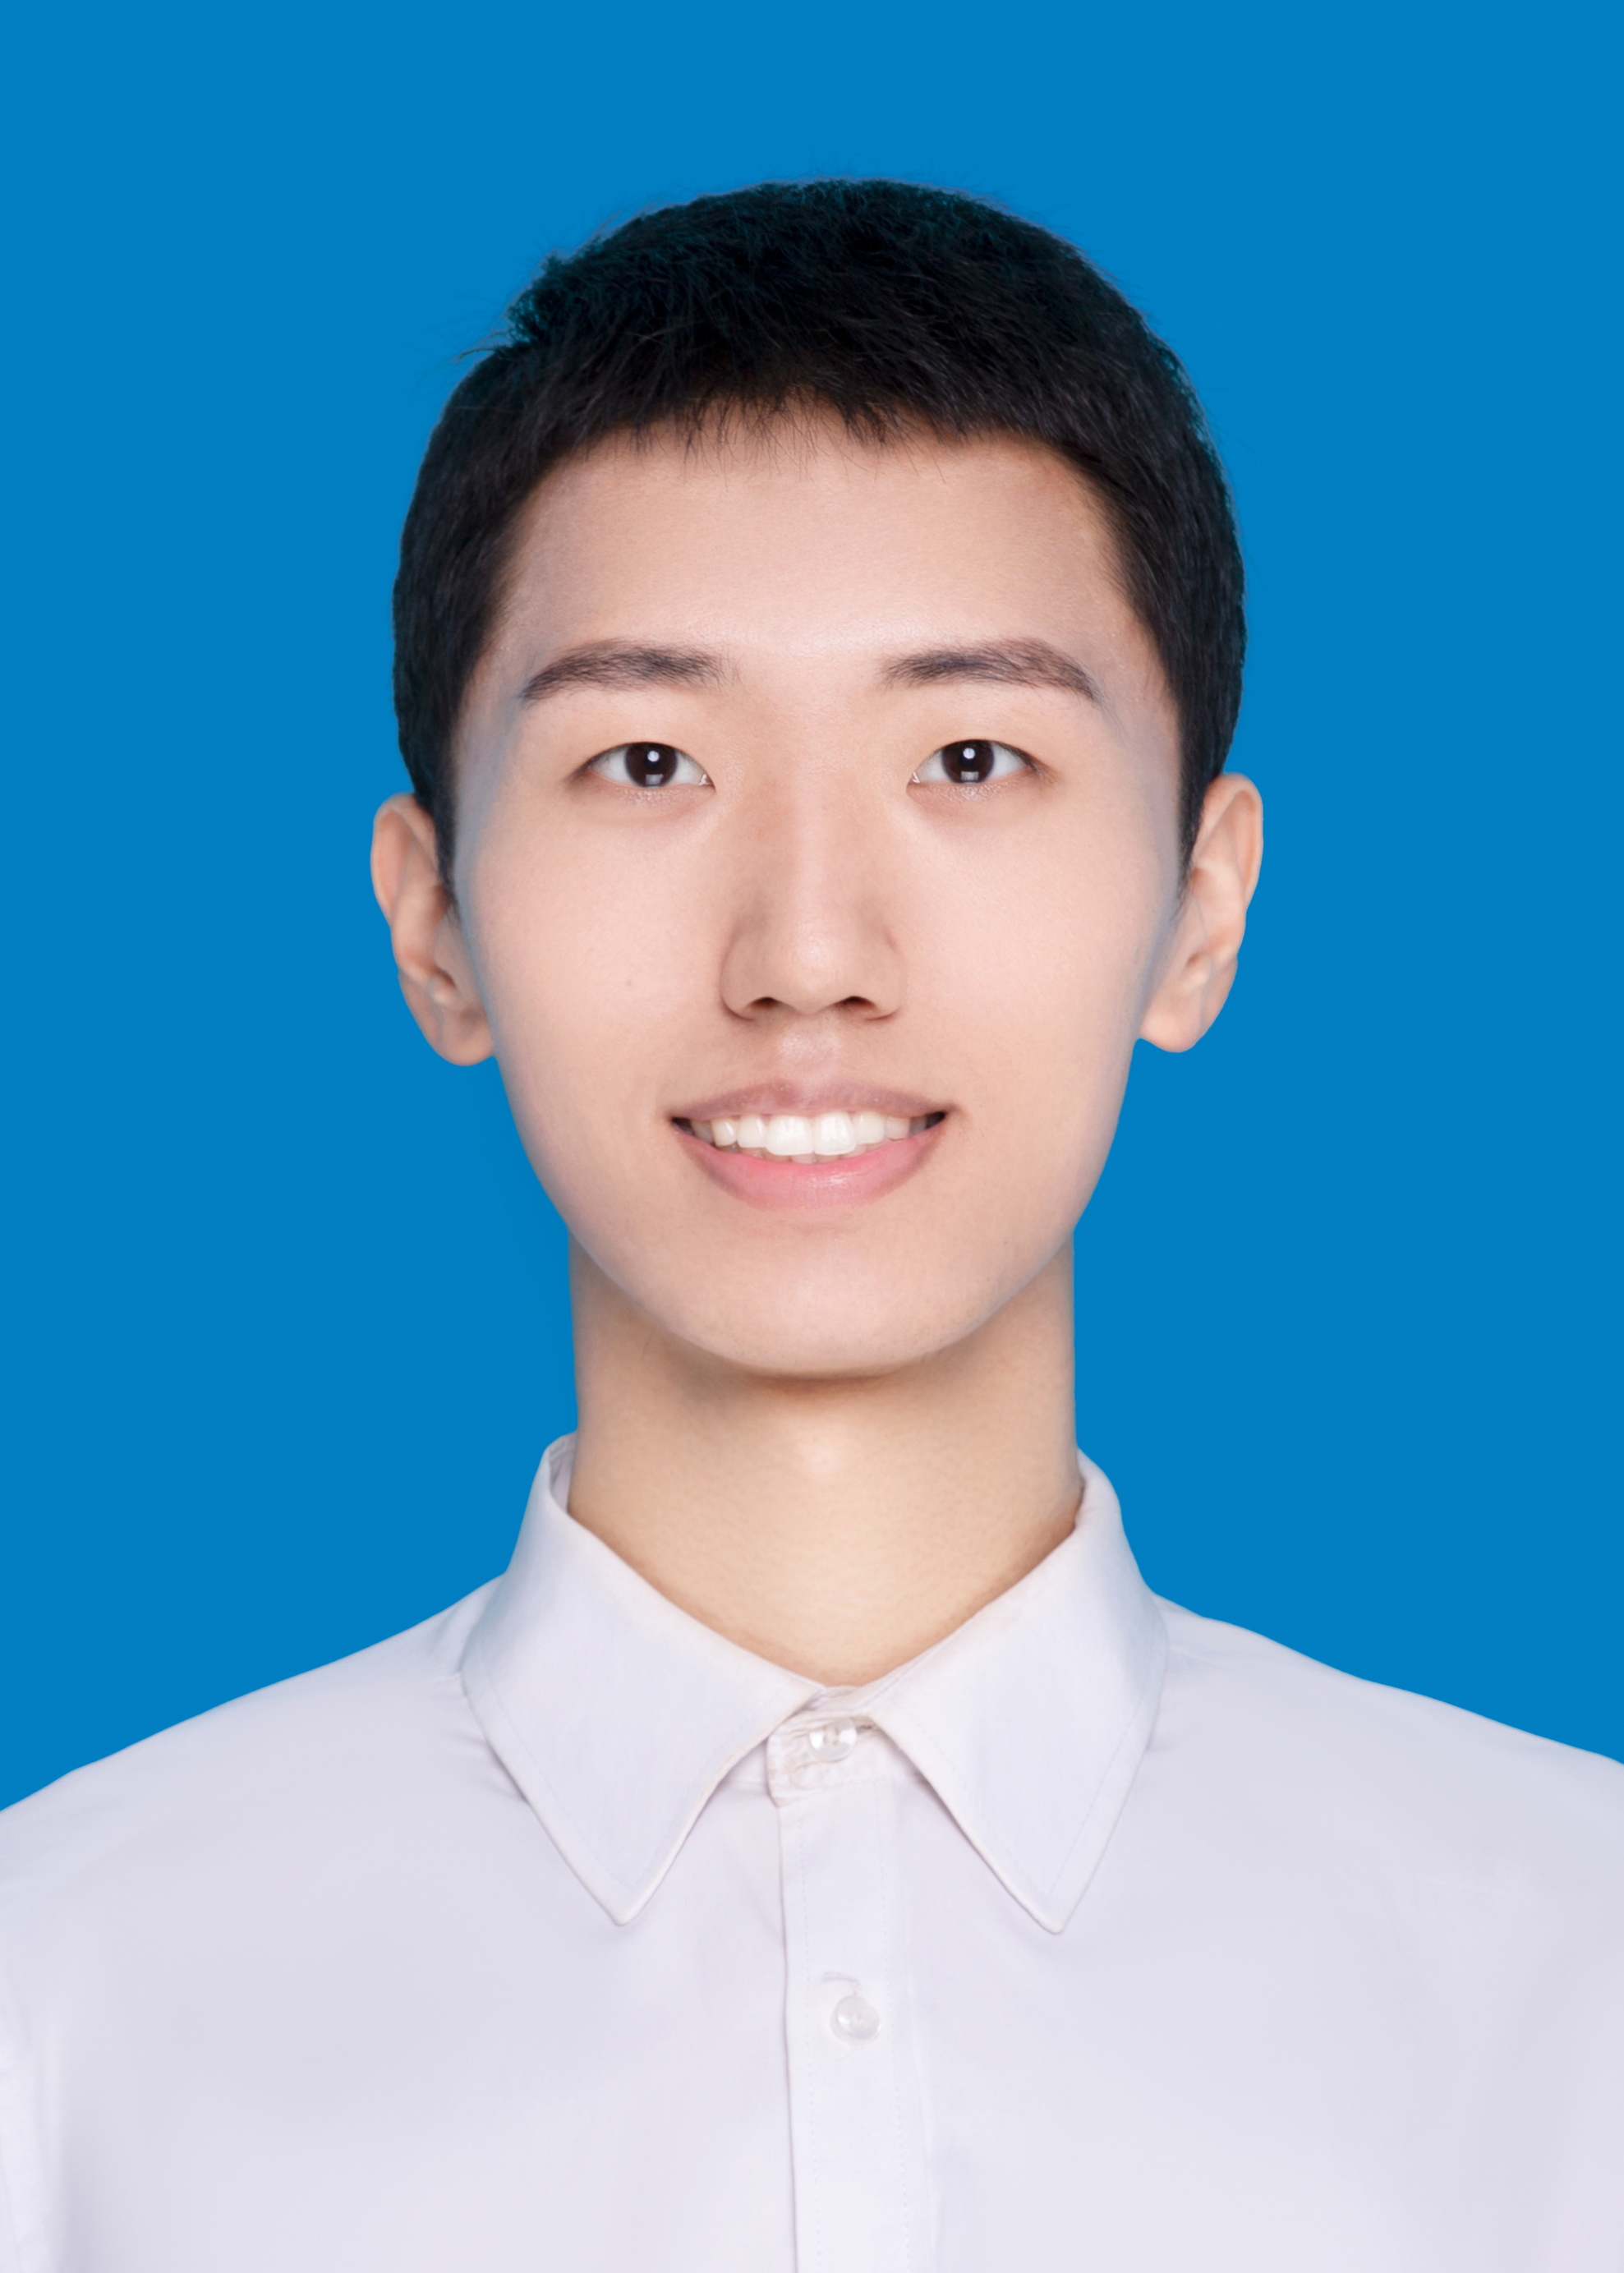
\includegraphics[width=2.8cm,height=3.6cm]{photo.jpg}}
\end{minipage}

\vspace{4pt}

% ===================== 教育背景 =====================
\section*{教育背景}

\eduentry{中国科学院大学}{高能物理研究所 \ 粒子物理与原子核物理}{硕士}{2023.09\,-\,至今}
\begin{itemize}
    \item GPA: 3.2/4
    \item 主要荣誉: 三好学生,国家奖学金,所长奖学金
    \item High-Performance Statistical Methods for Reactor Neutrino Oscillations, Eur. Phys. J C 85 (2025) 1420 (IF: 4.8,中科院二区),作者排名第一
    \item 英语水平: CET-4, CET-6
\end{itemize}

\eduentry{中北大学}{半导体与物理学院 \ 应用物理学}{本科}{2019.09\,-\,2023.06}
\begin{itemize}
    \item GPA: 4.30/5 \quad 排名: 1/100
    \item 保送研究生,获得校级"优秀毕业生",校长奖学提名奖(全院仅20名同学)、国家奖学金,连续两届全国数学竞赛省一等奖,全国大学生数学建模竞赛省二等奖,美国大学生数学建模竞赛H奖
\end{itemize}

% ===================== 科研项目 =====================
\section*{科研项目}

\begin{enumerate}[leftmargin=1.6em]
    \projitem{1}{算法优化与\textcolor{themered}{框架级重构}}{将JUNO实验反应堆中微子拟合算法进行\textbf{框架级重构},\textcolor{themered}{将谱预测}与似然评估张量化/批处理,显著减少循环与内存搬运,形成可在常规\textbf{算力稳定}运行的 FC 工程化流程,\textbf{整体加速约10倍},显著降低 CPU 成本。该框架已成功应用于反应堆中微子振荡分析,并可复用于其他基于正向折叠能谱的中微子实验,显著提升了 Feldman--Cousins 方法应用研究和大参数扫描的可行性。该项研究成果已在欧洲物理期刊C (Eur. Phys. J. C, 2025 IF: 4.8,中科院二区)发表,并在第25届江门中微子国际会议中做汇报。现已被高能所采纳用于\textbf{反应堆中微子振荡分析},并应用于 \textbf{JUNO首篇论文振荡分析}中。}

    \projitem{2}{大规模并行计算与模拟}{基于玩具蒙卡 (Toy MC) 研究统计偏差、Feldman-Cousins 方法。}
\end{enumerate}

\subproj{2.1}{基于玩具蒙卡实验研究了低统计量下不同分bin宽度下的拟合偏差,\textbf{增大重建能谱分bin宽度}可减小高斯近似 (CNP、Pearson统计方法) 下的拟合偏差,在100keV的bin宽下拟合偏差最小。基于此,JUNO 的首篇论文采用了100keV的bin宽来分bin。该工作在第26届江门中微子合作会议作报告。}

\subproj{2.2}{基于核数据库构建summation反应堆谱,并生成带有精细结构的变化谱。通过比较固定谱和变化谱,研究了\textbf{反应堆模型依赖}所引入的系统误差对振荡参数的影响。优化反应堆能谱分bin后,模型依赖对 $\sin^2\theta_{12}$、$\Delta m_{21}^2$ 的额外系统误差低于 \textbf{0.3\%},结果被JUNO实验首篇论文 \textbf{arXiv:2511.14593 [hep-ex]} 采纳,并在统计方法一节中讨论。}

\subproj{2.3}{针对低统计量下Wilks定理失效问题,使用\textbf{Feldman-Cousins方法}构建$\Delta\chi^2$分布,确保置信区间覆盖率正确。同时采用 \textbf{Feldman--Cousins} 方法研究振荡参数的统计性质,并评估了 Wilks \underline{近似在}不同参数下的适用性。结果表明,在 JUNO 首篇论文的统计量水平下,仅部分振荡参数满足 Wilks 定理。该工作为首篇论文中振荡参数结果的报告策略提供了统计依据,同时我还参与了JUNO实验首篇论文的振荡参数精确测量结果的交叉检验。}

\vspace{4pt}
\begin{enumerate}[leftmargin=1.6em,start=3]
    \projitem{3}{性能剖析与底层优化}{基于 Linux perf 与 Hotspot 对 JUNO omilrec 事例重建算法进行性能剖析,针对关键函数实施优化,最终将速度提升3倍。在第26届江门中微子国际合作会议中汇报。}
\end{enumerate}

% ===================== 学术会议及科研成果 =====================
\section*{学术会议及科研成果}

\begin{itemize}
    \item Jingqin Xue, Xuefeng Ding, et al ``High-Performance Statistical Methods for Reactor Neutrino Oscillations'' Eur. Phys. J. C 85 (2025) 1420, 作者排名第一
    \item Jingqin Xue, ``The accelerated reactor neutrino fitter and oscillation analysis of JUNO'' PoS, 作者排名第一
    \item Angel Abusleme, Thomas Adam, et al. ``First measurement of reactor neutrino oscillations at JUNO,'' arXiv e-prints, 2025. DOI: \url{https://doi.org/10.48550/arXiv.2511.14593}(合作组论文)
    \item Angel Abusleme, Thomas Adam, et al. ``Initial performance results of the JUNO detector,'' Chinese Physics C, 2026. DOI: \url{https://doi.org/10.1088/1674-1137/ae3dc1}.(合作组论文)
    \item 第二十五届江门中微子国际合作会议,主题报告《The accelerated reactor fitter》
    \item 第二十六届江门中微子国际合作会议,主题报告《Reducing Bias in Low exposure: Poisson method and binning strategies》
    \item 第二十六届江门中微子国际合作会议,主题报告《Speedup of OMILREC》
    \item 在TAUP2025会议上,做《The accelerated reactor fitter and Oscillation analysis for JUNO》poster
\end{itemize}

% ===================== 科研技能 =====================
\section*{科研技能}

\begin{description}[leftmargin=0pt,labelindent=0pt,style=unboxed,itemsep=3pt]
    \item[\textbf{编程语言与框架:}] 熟练掌握 C++、Python、PyTorch 等编程语言,熟悉代码运行内存管理与底层优化。
    \item[\textbf{性能调优与调试:}] Profiling Tools: 熟悉 Linux perf、Hotspot 工具的使用,具备针对底层代码优化的能力。
    \item[\textbf{开发配套与环境:}] Linux 生态: 熟练掌握 Shell 脚本、Makefile、CMake 构建系统,具备在集群环境下的分布式作业提交经验。版本控制与文档: 熟练使用 Git 进行协同开发与版本管理;精通 LaTeX 撰写\underline{高规范}学术及技术报告。
    \item[\textbf{AI效能与辅助开发:}] Vibe coding \& Writing: 熟练运用 Claude Code 等 Agentic 编程工具进行大规模代码库的重构与性能调优。利用 AI 工具进行高质量技术文档、学术论文(LaTeX)及项目提案的快速迭代。
\end{description}

\end{document}